% ============================================================
%  Práctica de Laboratorio 1 — Equipo ISA (Motor CC)
%  Control Automático — 2º Grado en ITT
%  Dpto. Ingeniería de Sistemas y Automática — Universidad de Sevilla
% ============================================================
\documentclass[12pt,a4paper]{article}
\usepackage[utf8]{inputenc}
\usepackage[T1]{fontenc}
\usepackage[spanish,es-nodecimaldot]{babel}
\usepackage{amsmath,amssymb}
\usepackage{graphicx}
\usepackage{tikz}
\usepackage{pgfplots}
\usepackage{booktabs}
\usepackage{array}
\usepackage{geometry}
\usepackage[colorlinks=true,linkcolor=blue!60!black,urlcolor=blue!60!black]{hyperref}
\usepackage{xcolor}
\usepackage{tcolorbox}
\usepackage{enumitem}
\usepackage{float}
\usepackage{caption}
\usepackage{subcaption}
\usepackage{fancyhdr}
\usepackage{multirow}
\usepackage{siunitx}
\usepackage{listings}

\usetikzlibrary{arrows.meta, positioning, fit, calc, shapes.geometric,
                shapes.misc, decorations.pathreplacing, backgrounds, matrix}
\pgfplotsset{compat=1.18}

\geometry{margin=2.5cm, top=3cm, bottom=3cm, headheight=14pt}

% ---- Colores corporativos ----
\definecolor{isablue}{RGB}{0,70,130}
\definecolor{isared}{RGB}{180,30,30}
\definecolor{lightgray}{RGB}{240,240,245}
\definecolor{answerbox}{RGB}{255,250,230}

% ---- Encabezado / pie ----
\pagestyle{fancy}
\fancyhf{}
\lhead{\small\textcolor{isablue}{\textbf{Control Automático — ITT}}}
\rhead{\small\textcolor{isablue}{\textbf{Práctica 1 — Equipo ISA}}}
\cfoot{\small\thepage}
\renewcommand{\headrulewidth}{0.4pt}

% ---- Caja de preguntas ----
\tcbuselibrary{skins,breakable}
\newtcolorbox{pregunta}[2][]{
  enhanced,
  colback=isared!8,
  colframe=isared,
  fonttitle=\bfseries\small,
  title={#2},
  #1
}

\newtcolorbox{notabox}{
  enhanced,
  colback=isablue!8,
  colframe=isablue,
  fonttitle=\bfseries\small,
  title={Nota},
}

% ---- Listings (código MATLAB) ----
\lstset{
  language=Matlab,
  basicstyle=\small\ttfamily,
  keywordstyle=\color{blue},
  commentstyle=\color{green!50!black}\itshape,
  stringstyle=\color{orange!80!black},
  numbers=left,
  numberstyle=\tiny\color{gray},
  frame=single,
  breaklines=true,
  captionpos=b
}

% ===========================================================
\begin{document}
% ===========================================================

% ---- Portada ----
\begin{center}
  \rule{\linewidth}{1.5pt}\\[6pt]
  {\LARGE\bfseries\color{isablue} Práctica 1}\\[6pt]
  {\Large Análisis de un motor de corriente continua}\\[4pt]
  \rule{\linewidth}{1.5pt}\\[8pt]
  {\small Dpto.\ de Ingeniería de Sistemas y Automática (ISA)\\[2pt]
   Universidad de Sevilla}
\end{center}

\vspace{6pt}

% ============================================================
\section{Objetivos}
% ============================================================

En esta práctica se va a familiarizar con el equipo de laboratorio basado en Arduino
diseñado por el grupo ISA, que permite controlar un motor de corriente continua
con lazo de control íntegramente en MATLAB/Simulink.
Los objetivos concretos son:

\begin{itemize}[noitemsep]
  \item Familiarizarse con el hardware y el modelo de Simulink del equipo.
  \item Leer la posición angular y la velocidad proporcionadas por el encoder magnético.
  \item Estudiar la calidad de la medida de velocidad y el efecto del filtrado.
  \item Identificar la función de transferencia del motor (ganancia estática~$K$ y
        constante de tiempo~$\tau$) mediante ensayos de escalón.
\end{itemize}

\begin{figure}[H]
\centering
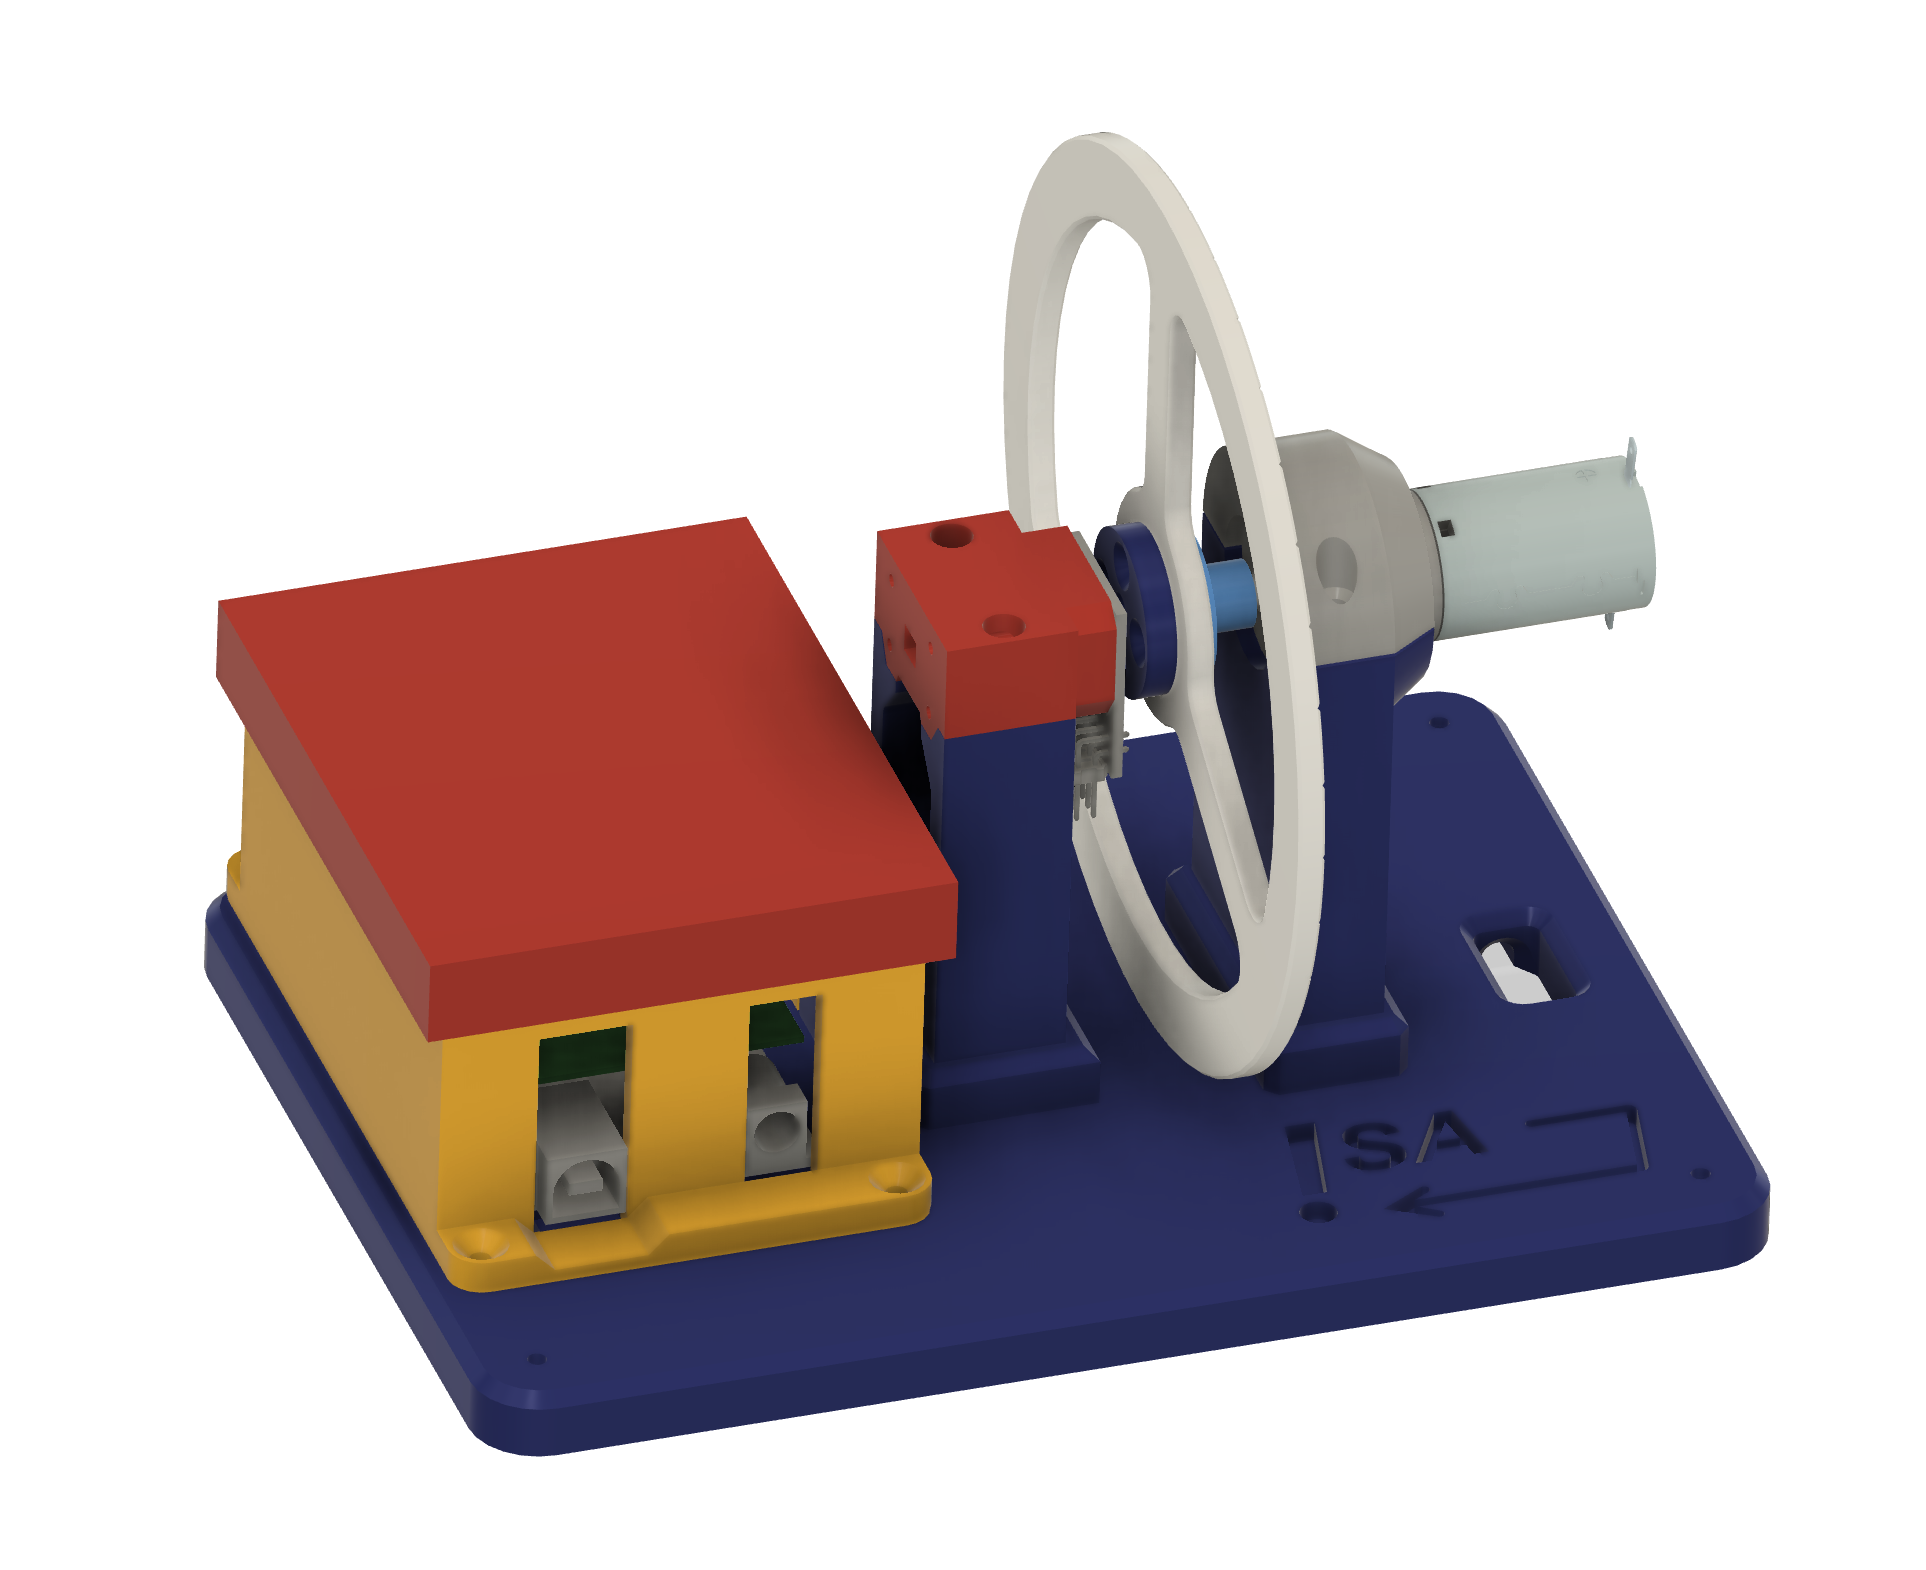
\includegraphics[width=0.55\linewidth]{../../docs/images/equipo_render.png}
\caption{Equipo de prácticas ISA: motor CC maxon A-max 22 con reductora GP~22B,
         encoder magnético AS5047P, driver TB6612FNG y Arduino UNO.}
\label{fig:equipo_foto}
\end{figure}

% ============================================================
\section{Descripción del equipo ISA}
% ============================================================

El banco de prácticas está formado por los siguientes elementos (figura~\ref{fig:esquema}):

\begin{itemize}[noitemsep]
  \item \textbf{Motor CC:} Maxon A-max~22, con reductora planetaria GP~22B.
  \item \textbf{Encoder:} AS5047P, encoder magnético absoluto de 14~bits
        ($2^{14}=16\,384$~pasos/vuelta), sin contacto y sin rozamiento.
  \item \textbf{Driver:} TB6612FNG, puente en H doble; permite PWM bipolar
        $u\in[-255,\,255]$.
  \item \textbf{Arduino UNO:} actúa como nodo de adquisición y actuación. Lee el encoder
        por SPI, calcula la velocidad y se comunica con el PC mediante protocolo
        serie binario a $\SI{115200}{baud}$, con período de muestreo
        $T_s=\SI{10}{ms}$ (100~Hz).
  \item \textbf{PC con MATLAB/Simulink:} ejecuta el algoritmo de control e
        intercambia datos con el Arduino a través del puerto USB/serie.
\end{itemize}

\begin{figure}[H]
\centering
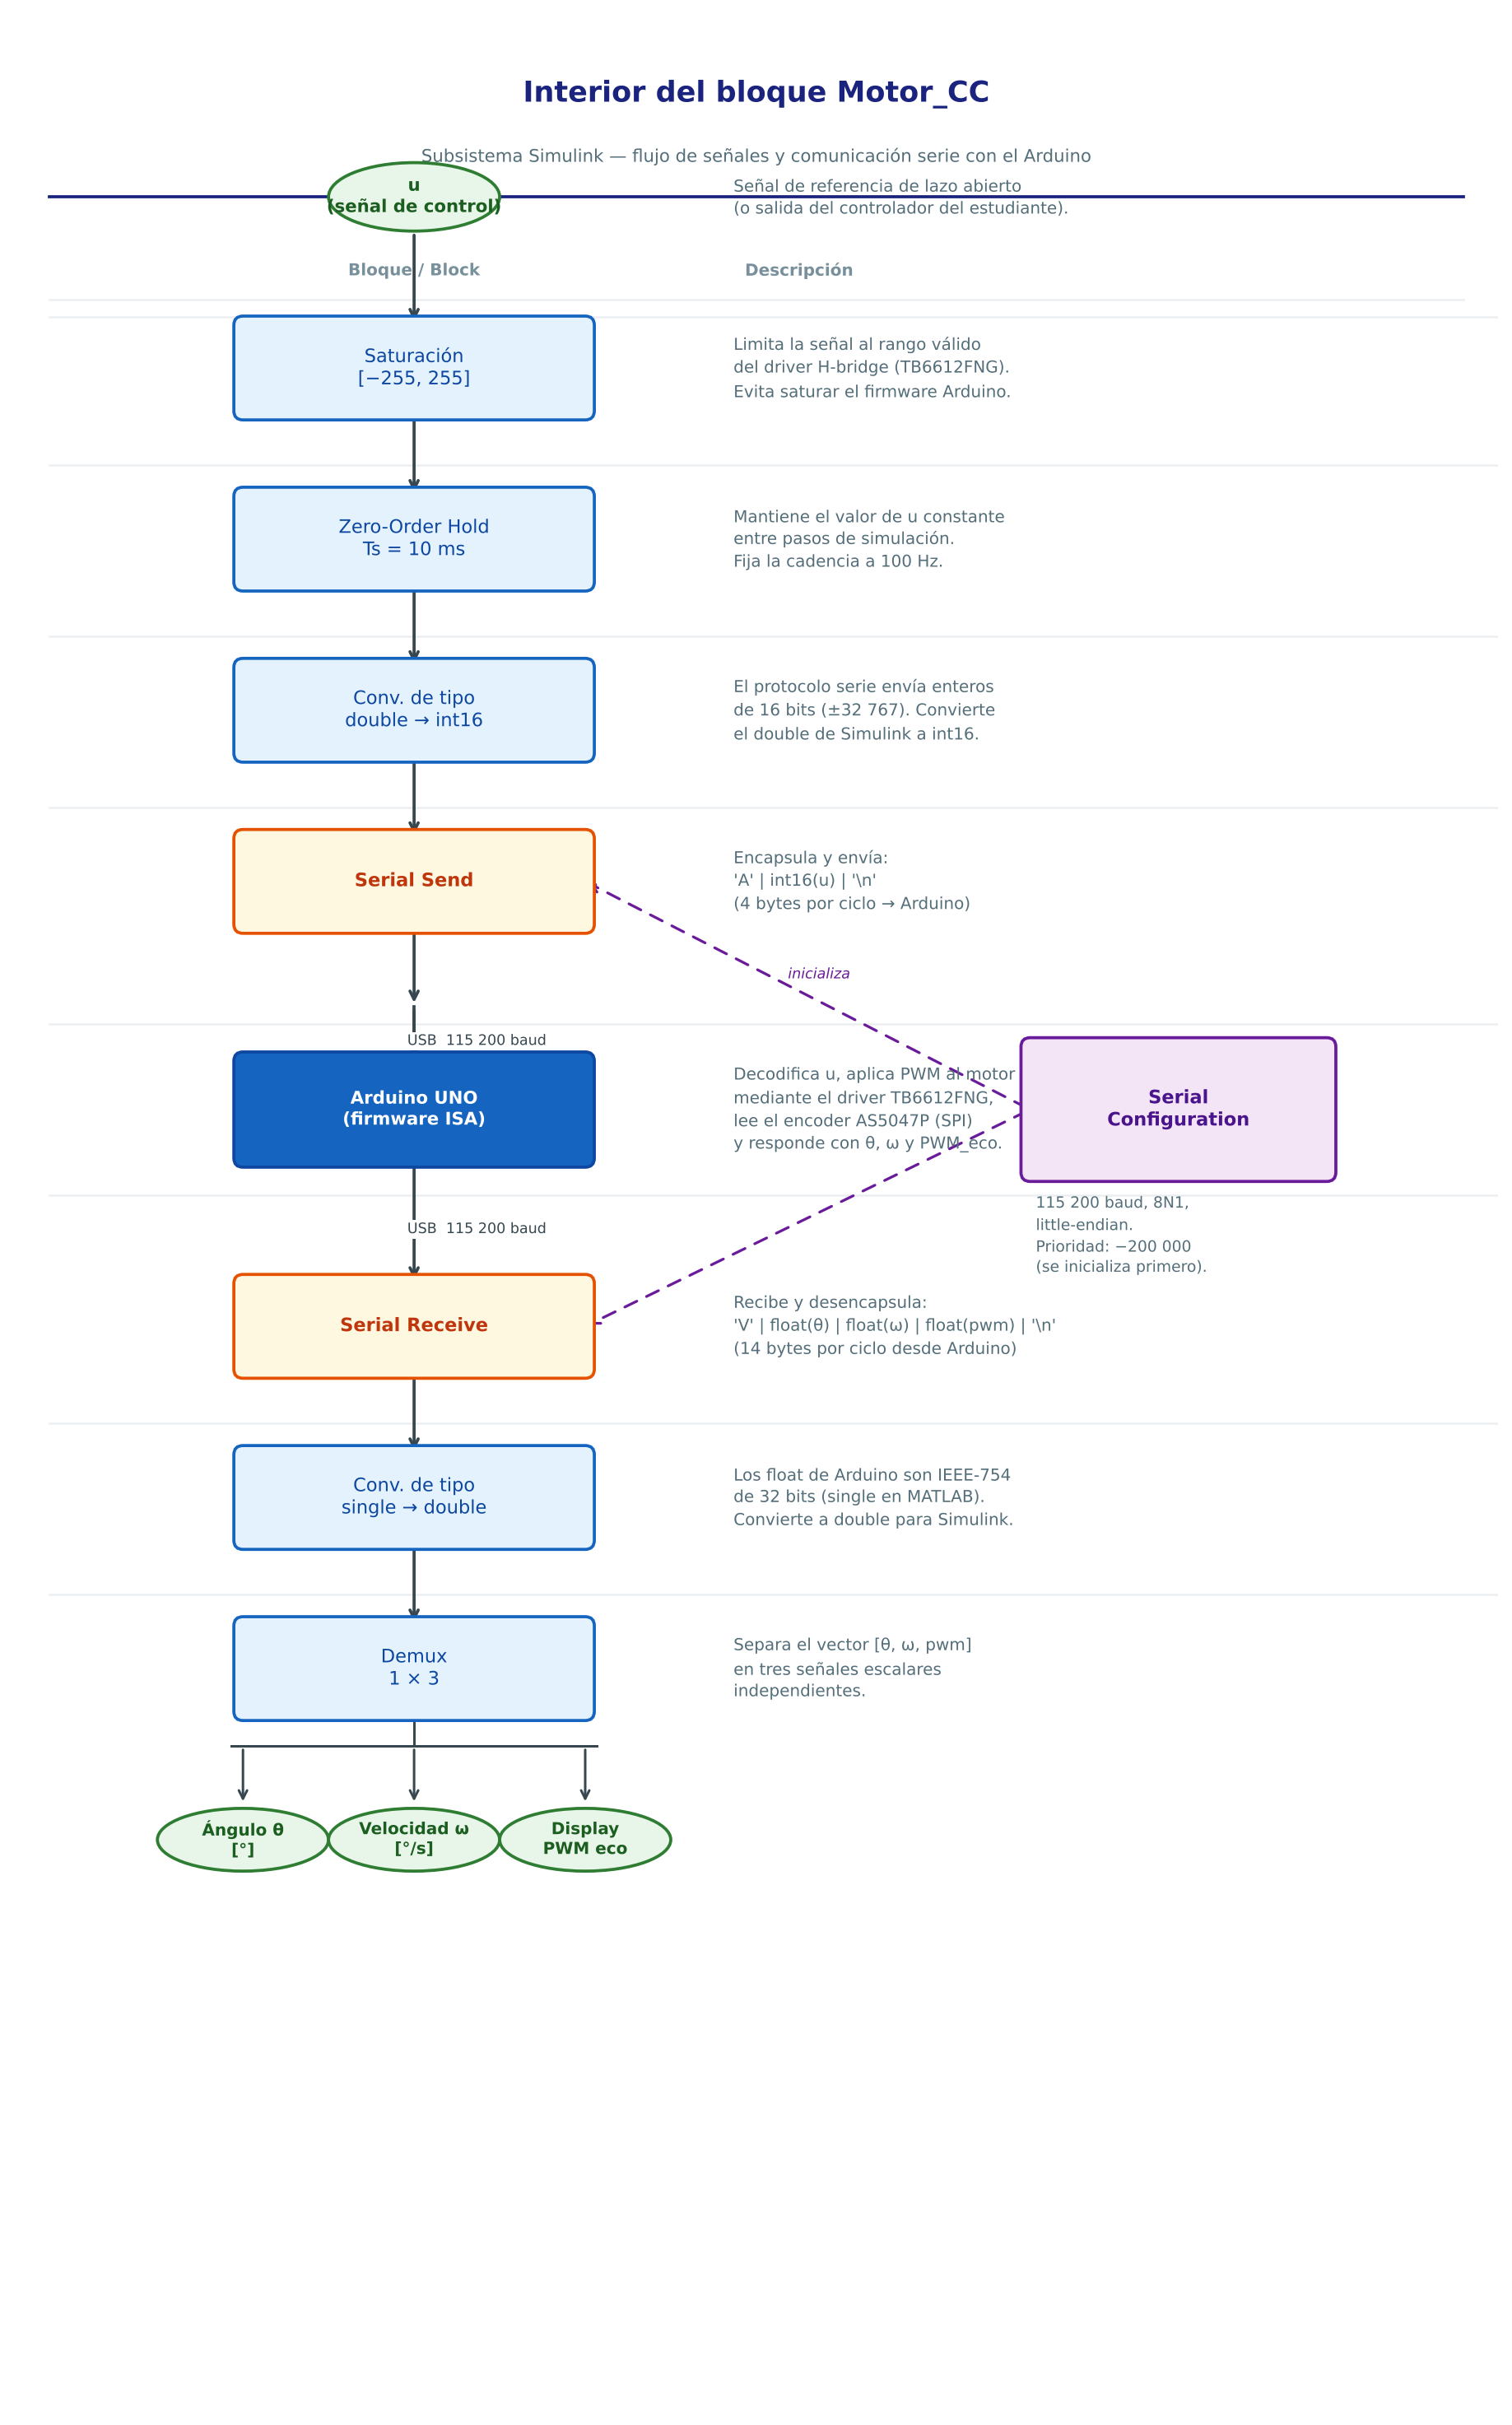
\includegraphics[width=0.92\linewidth]{../../docs/images/matlab/diagram_motor_cc_es.png}
\caption{Esquema del equipo de prácticas ISA.}
\label{fig:esquema}
\end{figure}

\subsection{Interfaz MATLAB -- Arduino}

El bloque \textbf{Motor\_CC} gestiona automáticamente la comunicación. Desde el
punto de vista del alumno, el intercambio es sencillo:

\begin{itemize}[noitemsep]
  \item \textbf{Simulink $\to$ Arduino:} cada 10~ms, el modelo envía al Arduino
        la señal de control~$u \in [-255,\;255]$.
        Un valor positivo gira el motor en un sentido; negativo, en el contrario.
        El valor~0 detiene el motor.
  \item \textbf{Arduino $\to$ Simulink:} el Arduino devuelve, también cada 10~ms,
        la posición angular acumulada~$\theta$ [°] y la velocidad angular~$\omega$ [°/s].
\end{itemize}

La relación entre la señal de control y la tensión equivalente aplicada al motor es:
\begin{equation}
  V_{eq} = u \cdot \frac{12\;\text{V}}{255}
  \qquad \Rightarrow \quad
  u = 255 \;\widehat{=}\; 12\;\text{V}, \quad u = 128 \;\widehat{=}\; 6\;\text{V}
  \label{eq:Veq}
\end{equation}

% ============================================================
\section{Puesta en marcha del equipo}\label{sec:puestaenmarcha}
% ============================================================

Toda la comunicación serie con el Arduino está encapsulada en el bloque
\textbf{Motor\_CC} del modelo \texttt{MotorCC\_V3.slx}. No es necesario
configurar ningún bloque serie manualmente; basta con seleccionar el puerto
al abrir el modelo.

\subsection{Pasos de puesta en marcha}

\begin{enumerate}
  \item \textbf{Conecte el Arduino al PC} mediante el cable USB.

  \item \textbf{Abra la carpeta del proyecto en MATLAB.}
        En el panel \emph{Current Folder} de MATLAB, navegue hasta el
        directorio \texttt{software/matlab/} del repositorio.

  \item \textbf{Abra el modelo.}
        Haga doble clic en \texttt{MotorCC\_V3.slx} en el explorador de
        archivos de MATLAB, o escriba en la consola:
        \begin{lstlisting}[numbers=none]
open('MotorCC_V3.slx')
        \end{lstlisting}

  \item \textbf{Seleccione el puerto serie.}
        Haga \textbf{doble clic} sobre el bloque \textbf{Motor\_CC} en el
        diagrama de Simulink. Se abrirá el diálogo de parámetros; el
        desplegable \emph{Puerto serie} mostrará automáticamente los puertos
        disponibles en el PC. Seleccione el que corresponde al Arduino
        (p.~ej., \texttt{COM3} en Windows, \texttt{/dev/tty.usbmodem\ldots}
        en macOS o \texttt{/dev/ttyACM0} en Linux) y pulse \emph{OK}.

  \item \textbf{Pulse \emph{Run}.}
        Haga clic en el botón \textbf{Run} (\raisebox{-1pt}{\(\triangleright\)})
        de la barra de herramientas de Simulink. El modelo se ejecuta en
        \emph{tiempo real}, sincronizado con el Arduino a 100~Hz.

  \item \textbf{Verifique el funcionamiento.}
        El Scope debe mostrar señales de ángulo~$\theta$ y velocidad~$\omega$
        que varían en tiempo real. Si el motor no gira o el Scope no actualiza,
        compruebe:
        \begin{itemize}[noitemsep]
          \item que el Arduino está encendido (LED de alimentación visible),
          \item que ha seleccionado el puerto correcto en el bloque Motor\_CC,
          \item que la alimentación del motor~(12~V) está conectada.
        \end{itemize}
\end{enumerate}

\begin{notabox}
  Una vez seleccionado el puerto, el modelo lo recuerda hasta la próxima vez
  que se abra. Solo hay que volver al diálogo del bloque si se cambia de
  ordenador o de puerto USB.
\end{notabox}

\subsection{Entradas y salidas del bloque Motor\_CC}

\begin{figure}[H]
\centering
\begin{tikzpicture}[
  bigblock/.style={draw=isablue, fill=isablue!12, minimum width=3.5cm,
                   minimum height=3.2cm, align=center, font=\small\bfseries,
                   rounded corners=4pt, line width=1.2pt},
  port/.style={font=\scriptsize},
  arr/.style={-{Stealth[length=5pt]}, thick}
]
  \node[bigblock] (motor) {Motor\_CC};

  % Entrada
  \node[port, left=2.2cm of motor] (u_in) {$u\;[-255,\,255]$};
  \draw[arr] (u_in) -- node[above,font=\scriptsize]{señal de\\[-3pt]control} (motor.west);

  % Salidas
  \node[port, right=2.4cm of motor, yshift= 0.9cm] (th) {$\theta$ [°]};
  \node[port, right=2.4cm of motor, yshift= 0.0cm] (om) {$\omega$ [°/s]};
  \node[port, right=2.4cm of motor, yshift=-0.9cm] (pw) {$u_{eco}$ [-255,255]};

  \draw[arr] (motor.east |- th) -- (th);
  \draw[arr] (motor.east |- om) -- (om);
  \draw[arr] (motor.east |- pw) -- (pw);

  % Notas
  \node[font=\tiny, below=0.15cm of motor] {(encapsula Serial Config, Send y Receive)};
\end{tikzpicture}
\caption{Bloque Motor\_CC: entrada (señal de control $u$) y salidas (posición $\theta$,
velocidad $\omega$ y eco de la señal de control).}
\label{fig:motor_cc_block}
\end{figure}

El modelo base ya incluye una entrada \emph{Constant} (valor~50) y un bloque
\emph{Scope} conectados al bloque Motor\_CC. Puede modificar el valor de la
constante y conectar bloques adicionales según necesite en cada apartado.

\begin{notabox}
  El motor gira en ambas direcciones según el signo de~$u$.
  Comience con valores pequeños ($|u|\leq 50$) para evitar golpes bruscos.
  La simulación se ejecuta en tiempo real sincronizada con el Arduino.
\end{notabox}

% ============================================================
\section{Verificación del equipo}
% ============================================================

Antes de comenzar los apartados de medida, compruebe que el equipo funciona
correctamente siguiendo estos pasos:

\begin{enumerate}
  \item Asegúrese de haber completado la puesta en marcha de la
        sección~\ref{sec:puestaenmarcha} (Arduino conectado, puerto seleccionado).

  \item En el modelo de Simulink, haga doble clic sobre el bloque \textbf{Constant}
        y fije su valor a $u = 50$.

  \item Ajuste el tiempo de parada de la simulación a \textbf{5~s} en la barra de
        herramientas (\emph{Stop Time}).

  \item Pulse \textbf{Run}. El motor debe girar a velocidad aproximadamente constante.
        El Scope debe mostrar:
        \begin{itemize}[noitemsep]
          \item $\theta$: una rampa creciente (el eje gira acumulando ángulo).
          \item $\omega$: una señal aproximadamente constante, con pequeñas
                fluctuaciones debidas al ruido del encoder.
        \end{itemize}

  \item Espere a que la simulación termine (5~s) o pulse \textbf{Stop}.
        Cambie $u = -50$ y vuelva a pulsar \textbf{Run}: el motor debe girar
        en sentido contrario ($\theta$ decrece, $\omega$ es negativo).

  \item Fije $u = 0$ y compruebe que el motor se detiene (puede tardar unos
        instantes por inercia).
\end{enumerate}

\begin{notabox}
  Si el motor no gira pero el Scope sí muestra señales, compruebe la alimentación
  de 12~V del driver. Si el Scope no muestra nada, vuelva al bloque Motor\_CC
  y verifique el puerto serie seleccionado.
\end{notabox}

% ============================================================
\section{Señal de actuación y lectura del sensor}
% ============================================================

Una vez verificado el funcionamiento, en este apartado va a medir la respuesta del
motor ante distintas señales de control.

\begin{enumerate}
  \item Configure el bloque \emph{Constant} con el valor $u = 50$.
  \item Ajuste el tiempo de parada de la simulación a $\SI{5}{s}$ en la barra de
        herramientas de Simulink.
  \item Pulse \textbf{Run}. El scope debe mostrar el ángulo y la velocidad del motor.
  \item Repita con $u = -50$ y con $u = 0$.
\end{enumerate}

\begin{pregunta}{Pregunta \#1 — Resolución del encoder}
  \begin{enumerate}[label=\alph*)]
    \item ¿Cuántos pasos da el encoder AS5047P por revolución?
    \item Calcule la resolución en grados y en radianes por paso.
    \item El Arduino envía el ángulo acumulado en grados. Si se desea trabajar en
          radianes, ¿qué factor de conversión hay que aplicar en Simulink?
  \end{enumerate}
\end{pregunta}

\begin{pregunta}{Pregunta \#2 — Señal de actuación y velocidad en régimen permanente}
  Con $u = 50$:
  \begin{enumerate}[label=\alph*)]
    \item ¿Cuál es la velocidad en régimen permanente en °/s?
    \item Convierta ese valor a rad/s.
    \item ¿Qué tensión equivalente $V_{eq}$ [V] corresponde a $u = 50$?
    \item ¿Qué ocurre si invierte el signo de $u$? ¿Y si pone $u = 0$?
  \end{enumerate}
\end{pregunta}

% ============================================================
\section{Medida de velocidad}
% ============================================================

El Arduino calcula la velocidad como la variación de ángulo entre dos períodos consecutivos:
\begin{equation}
  \omega[k] = \frac{\theta[k] - \theta[k-1]}{T_s} \quad [\si{\degree/s}]
  \label{eq:vel_discreta}
\end{equation}
con $T_s = \SI{10}{ms}$. Esta diferencia discreta amplifica el ruido de cuantificación del encoder.

\subsection{Observación del ruido de velocidad}

\begin{enumerate}
  \item Aplique $u = 50$ y observe en el Scope la señal de velocidad $\omega$ en
        régimen permanente. Haga zoom en unos pocos ciclos para apreciar la
        variación de muestra a muestra.
  \item Estime visualmente la amplitud pico a pico del ruido de velocidad.
\end{enumerate}

\subsection{Filtrado paso bajo de la velocidad}

Para atenuar el ruido, se puede añadir un filtro paso bajo de primer orden en Simulink:
\begin{equation}
  F(s) = \frac{\omega_c}{s + \omega_c}
  \label{eq:filtro}
\end{equation}

Añada un bloque \emph{Transfer Fcn} entre la salida $\omega$ del bloque Motor\_CC
y el Scope, con numerador $[\omega_c]$ y denominador $[1,\;\omega_c]$.
Pruebe con $\omega_c = 50\;\si{rad/s}$ (frecuencia de corte $\approx 8\;\si{Hz}$).

\begin{notabox}
  Recuerde establecer el tiempo de muestreo del bloque Transfer Fcn en $-1$
  (hereda del solver). El solver de Simulink debe ser de paso fijo con
  $T_{step} = \SI{0.01}{s}$.
\end{notabox}

\begin{pregunta}{Pregunta \#3 — Calidad de la medida de velocidad}
  \begin{enumerate}[label=\alph*)]
    \item ¿Cuál es la resolución mínima de velocidad que puede detectar el encoder
          para $T_s = \SI{10}{ms}$? (Recuerde: 16\,384~pasos/vuelta.)
    \item Compare cualitativamente la señal de velocidad sin filtrar y con el filtro
          $F(s)=50/(s+50)$: ¿qué mejora se observa en el ruido? ¿Y qué retardo
          introduce el filtro?
    \item ¿Qué criterio usaría para elegir $\omega_c$? Razone en términos de
          compromiso entre atenuación de ruido y retardo.
  \end{enumerate}
\end{pregunta}

% ============================================================
\section{Identificación de la función de transferencia}
% ============================================================

Se va a identificar el modelo de primer orden del motor usando ensayos de escalón:
\begin{equation}
  G(s) = \frac{\Omega(s)}{V_{eq}(s)} = \frac{K}{\tau s + 1}
  \label{eq:tf}
\end{equation}
donde $\Omega(s)$ es la velocidad en rad/s, $V_{eq}(s)$ es la tensión equivalente
en voltios, $K$~[\si{rad.s^{-1}.V^{-1}}] es la ganancia estática y $\tau$~[\si{s}]
la constante de tiempo.

\subsection{Procedimiento}

\begin{enumerate}
  \item Modifique el modelo para que el bloque \emph{Constant} proporcione la
        señal de control. Para el ensayo de escalón, utilice $u = 50$
        (equivalente a $V_{eq} \approx \SI{2.35}{V}$).
  \item Añada una conversión a rad/s multiplicando la salida $\omega$ por
        $\pi/180$ (bloque \emph{Gain}).
  \item Configure la simulación para al menos $\SI{2}{s}$ de duración.
  \item Ejecute la simulación partiendo del motor en reposo.
  \item Exporte los datos del Scope a MATLAB pulsando el botón
        \emph{Log/unlog signals} o usando \texttt{simout} con un bloque
        \emph{To Workspace}.
\end{enumerate}

\subsection{Determinación gráfica de $K$ y $\tau$}

A partir de la respuesta al escalón (figura~\ref{fig:step_response}):

\begin{itemize}[noitemsep]
  \item \textbf{Ganancia estática:}
        \begin{equation}
          K = \frac{\omega_{ss}}{V_{eq}}
          \label{eq:K}
        \end{equation}
        donde $\omega_{ss}$ es la velocidad en régimen permanente.
  \item \textbf{Constante de tiempo:}
        $\tau$ es el tiempo que tarda la velocidad en alcanzar
        el $63.2\%$ de $\omega_{ss}$ desde el inicio del escalón.
\end{itemize}

\begin{figure}[H]
\centering
\begin{tikzpicture}
\begin{axis}[
  width=12cm, height=6cm,
  xlabel={Tiempo [s]},
  ylabel={Velocidad $\omega$ [rad/s]},
  xmin=0, xmax=1.0,
  ymin=0, ymax=28,
  grid=both,
  grid style={line width=0.3pt, draw=gray!30},
  major grid style={line width=0.6pt, draw=gray!60},
  tick label style={font=\small},
  label style={font=\small},
  legend style={font=\small, at={(0.6,0.3)}, anchor=west},
]
  % Respuesta al escalón de primer orden: wss=24, tau=0.07, inicio en t=0.1
  \addplot[thick, color=isablue, domain=0:0.1, samples=5] {0};
  \addplot[thick, color=isablue, domain=0.1:1.0, samples=100]
    {24*(1 - exp(-(x-0.1)/0.07))};

  % Línea de régimen permanente
  \addplot[dashed, color=isared, domain=0:1.0] {24}
    node[right, font=\scriptsize] {$\omega_{ss}$};

  % 63.2%
  \addplot[dashed, color=gray, domain=0:1.0] {0.632*24}
    node[right, font=\scriptsize] {$0.632\,\omega_{ss}$};

  % Marca de tau
  \draw[{Stealth[length=5pt]}-{Stealth[length=5pt]}, gray]
    (axis cs:0.1,2) -- (axis cs:0.17,2)
    node[midway, above, font=\scriptsize] {$\tau$};

  \addlegendentry{$\omega(t)$ (medida)};
\end{axis}
\end{tikzpicture}
\caption{Respuesta al escalón de velocidad. Se identifican gráficamente
la velocidad en régimen permanente $\omega_{ss}$ y la constante de tiempo $\tau$.}
\label{fig:step_response}
\end{figure}

\begin{pregunta}{Pregunta \#4 — Función de transferencia (con y sin reductora)}
  \begin{enumerate}[label=\alph*)]
    \item Aplique el escalón $u=50$ ($V_{eq}\approx\SI{2.35}{V}$) y
          determine $\omega_{ss}$ en rad/s.
    \item Calcule la ganancia estática $K$ usando la ecuación~(\ref{eq:K}).
    \item Determine $\tau$ gráficamente a partir de la curva de respuesta.
    \item Escriba la función de transferencia $G(s) = K/(\tau s + 1)$ con los
          valores obtenidos.
  \end{enumerate}
\end{pregunta}

\begin{pregunta}{Pregunta \#5 — Validación del modelo}
  \begin{enumerate}[label=\alph*)]
    \item Repita el ensayo con $u=-50$. ¿Es el sistema simétrico?
          ¿Obtiene los mismos valores de $K$ y $\tau$?
    \item Repita con $u=100$. ¿Se mantiene la linealidad? Razone la respuesta.
    \item Usando la función de transferencia identificada y la herramienta
          \texttt{step} de MATLAB (o el bloque Transfer Fcn en Simulink),
          superponga la respuesta del modelo sobre la medida experimental.
          ¿El ajuste es satisfactorio?
  \end{enumerate}
\end{pregunta}

\begin{pregunta}{Pregunta \#6 — Efecto de la reductora}
  El motor lleva acoplada una reductora planetaria GP~22B. ¿Cómo afecta
  la reductora a la constante de tiempo $\tau$ y a la ganancia estática $K$
  en comparación con un motor sin reductora? Razone cualitativamente.
\end{pregunta}

% ============================================================
\section*{Hoja de respuestas}
% ============================================================
\addcontentsline{toc}{section}{Hoja de respuestas}

\begin{center}
{\large\bfseries Hoja de respuestas — Práctica 1}
\end{center}

Nombre: \underline{\hspace{8cm}}

\vspace{6pt}

\begin{tabular}{|p{5.5cm}|p{8.5cm}|}
\hline
\multicolumn{1}{|c|}{\textbf{Dato solicitado}} &
\multicolumn{1}{c|}{\textbf{Respuesta}} \\
\hline
\#1 Resolución del encoder &
\vspace{2.5cm} \\
\hline
\#2 Velocidad en régimen permanente ($u=50$) &
\vspace{2.5cm} \\
\hline
\#3 Calidad de la medida de velocidad &
\vspace{2.5cm} \\
\hline
\#4 Función de transferencia $G(s)$ &
\vspace{2.5cm} \\
\hline
\#5 Validación del modelo &
\vspace{2.5cm} \\
\hline
\#6 Efecto de la reductora &
\vspace{2.5cm} \\
\hline
\end{tabular}

% ============================================================
\appendix
\section{El encoder magnético AS5047P}
% ============================================================

A diferencia de los encoders ópticos incrementales, el AS5047P es un encoder
\textbf{magnético absoluto} de 14~bits. Sus principales características son:

\begin{itemize}[noitemsep]
  \item \textbf{Resolución:} $2^{14} = 16\,384$ posiciones por vuelta
        $\Rightarrow$ resolución de $360/16\,384 \approx 0.022\,°/\text{paso}$.
  \item \textbf{Lectura absoluta:} No necesita referencia inicial (homing) ni
        contador de pulsos; devuelve el ángulo directamente en cada lectura SPI.
  \item \textbf{Sin contacto:} El sensor lee el campo magnético de un imán
        solidario al eje; no hay desgaste mecánico ni rozamiento.
  \item \textbf{Interfaz:} SPI a hasta 10~MHz (el firmware usa 400~kHz para
        mayor robustez).
\end{itemize}

El firmware de Arduino acumula el ángulo entre vueltas para proporcionar una
posición angular absoluta ilimitada:
\begin{equation}
  \theta_{abs}[k] = \theta_{raw}[k] + 360 \cdot n_{vueltas}
\end{equation}
donde $\theta_{raw}\in[-180°,180°)$ y $n_{vueltas}$ se actualiza cada vez que
se detecta un cruce por $\pm 180°$.

La velocidad se calcula directamente en el firmware como:
\begin{equation}
  \omega[k] = \frac{\theta_{abs}[k] - \theta_{abs}[k-1]}{T_s}
  \quad [\si{\degree/s}], \quad T_s = \SI{10}{ms}
\end{equation}

\end{document}
